\documentclass[aspectratio=169]{beamer}

% ── Tema base ─────────────────────────────────────────────────────────────────
\usetheme{default}
\usecolortheme{default}
\setbeamertemplate{navigation symbols}{}

% ── Colores UTEC ──────────────────────────────────────────────────────────────
\definecolor{utecblue}{RGB}{0,82,155}
\definecolor{uteccyan}{RGB}{0,174,219}
\definecolor{lightgray}{RGB}{245,245,245}

\setbeamercolor{frametitle}{bg=utecblue, fg=white}
\setbeamerfont{frametitle}{size=\large, series=\bfseries}

\setbeamercolor{title}{fg=white}
\setbeamercolor{subtitle}{fg=uteccyan}
\setbeamercolor{author}{fg=white}
\setbeamercolor{institute}{fg=white!80}
\setbeamercolor{date}{fg=white!70}

\setbeamercolor{block title}{bg=utecblue, fg=white}
\setbeamercolor{block body}{bg=utecblue!8, fg=black}
\setbeamercolor{alertblock title}{bg=uteccyan!80!black, fg=white}
\setbeamercolor{alertblock body}{bg=uteccyan!12, fg=black}

\setbeamercolor{itemize item}{fg=utecblue}
\setbeamercolor{itemize subitem}{fg=uteccyan}
\setbeamertemplate{itemize item}{\small$\blacktriangleright$}
\setbeamertemplate{itemize subitem}{\small$\triangleright$}

\setbeamertemplate{footline}{%
  \hfill\usebeamerfont{footline}\insertframenumber\,/\,\inserttotalframenumber\hspace{1em}\vspace{0.4em}
}

\setbeamercolor{background canvas}{bg=white}

% ── Paquetes ──────────────────────────────────────────────────────────────────
\usepackage[utf8]{inputenc}
\usepackage[T1]{fontenc}
\usepackage{graphicx}
\usepackage{booktabs}
\usepackage{amsmath}
\usepackage{amssymb}
\usepackage{tikz}
\usepackage{array}
\usepackage{colortbl}
\usepackage{pgfplots}
\usepackage{xcolor}
\usepackage{url}
\pgfplotsset{compat=1.18}
\usetikzlibrary{arrows.meta, shapes.geometric, positioning, fit, backgrounds}

% ── Comando para placeholder de imagen/video ──────────────────────────────────
\newcommand{\imgplaceholder}[2][8cm]{%
  \begin{tikzpicture}
    \node[draw=utecblue!40, dashed, fill=utecblue!5,
          minimum width=#1, minimum height=4cm,
          font=\small\color{utecblue!70}, align=center,
          rounded corners=4pt] {#2};
  \end{tikzpicture}%
}

% ── Metadatos ─────────────────────────────────────────────────────────────────
\title{Multi-Object Tracking in UAV Imagery}
\subtitle{Method 1 (Baseline): YOLOv11 + SORT}
\author{Rensso Victor Hugo Mora Colque}
\institute{Computer Vision --- UTEC}
\date{2026-I}

% =============================================================================
\begin{document}
% =============================================================================

% ── SLIDE 1: PORTADA ──────────────────────────────────────────────────────────
{
\setbeamercolor{background canvas}{bg=white}
\begin{frame}[plain]
  \vspace{1.2cm}
  \centering
  {\color{utecblue}\Large\bfseries Multi-Object Tracking in UAV Imagery\par}
  \vspace{0.4em}
  {\color{uteccyan}\normalsize Method 1 (Baseline): YOLOv11 + SORT\par}
  \vspace{1.2em}
  \color{utecblue!50}\rule{0.5\textwidth}{0.4pt}\par
  \vspace{0.8em}
  {\color{utecblue!80}\small Computer Vision --- UTEC\par}
  {\color{utecblue!80}\small Assignment IV: Detection and Tracking\par}
  \vspace{0.4em}
  {\color{utecblue!70}\small Rensso Victor Hugo Mora Colque\par}
  {\color{utecblue!60}\small 2026-I\par}
\end{frame}
}

% ── SLIDE 2: MOTIVACIÓN ───────────────────────────────────────────────────────
\begin{frame}{Motivation and Context}
  \begin{columns}[T]
    \begin{column}{0.55\textwidth}
      \textbf{Why MOT in UAV/drone imagery?}
      \begin{itemize}
        \item Surveillance, traffic management, search \& rescue
        \item Drones provide flexible, wide-area coverage
        \item Unique challenges vs.\ ground-level cameras:
              \begin{itemize}
                \item Objects appear at \textbf{very small scales} ($<20$ px)
                \item High \textbf{target density} and frequent occlusion
                \item Significant \textbf{camera ego-motion}
              \end{itemize}
      \end{itemize}
      \vspace{0.4em}
      \begin{alertblock}{Core approach: tracking-by-detection}
        \small Decouple detection and association.
        A detector produces per-frame bounding boxes;
        a tracker links them into persistent trajectories.
      \end{alertblock}
    \end{column}
    \begin{column}{0.40\textwidth}
      \begin{block}{Pipeline overview}
        \small
        \textbf{1.}~Frame $t$ (JPEG image)\\
        $\downarrow$~\textit{YOLOv11 detector}\\
        \textbf{2.}~Bounding boxes $\{b_i^t\}$\\
        $\downarrow$~\textit{SORT tracker}\\
        \textbf{3.}~Trajectories $\{\tau_k\}$\\
        $\downarrow$~\textit{motmetrics}\\
        \textbf{4.}~MOTA, IDF1, IDS, FPS
      \end{block}
      \vspace{0.3em}
      \begin{block}{Classes evaluated}
        \small
        \textbf{Class 1} Pedestrian \quad
        \textbf{Class 4} Car\\
        {\footnotesize(VisDrone-MOT annotation format)}
      \end{block}
    \end{column}
  \end{columns}
\end{frame}

% ── SLIDE 3: DATASET ──────────────────────────────────────────────────────────
\begin{frame}{Dataset: VisDrone2019-MOT-val}
  \begin{columns}[T]
    \begin{column}{0.52\textwidth}
      \textbf{Dataset characteristics \cite{zhu2022visdrone}:}
      \begin{itemize}
        \item Captured by DJI drones over 14 cities in China
        \item 10 object categories (pedestrian, car, van, bus, \ldots)
        \item Ground-truth format (MOT standard, 10 fields):
      \end{itemize}
      \vspace{0.2em}
      {\footnotesize
        \texttt{frame, id, x, y, w, h, score, class, trunc, occl}}
      \vspace{0.3em}
      \begin{alertblock}{Restriction in this work}
        \small Filter only \textbf{class 1} (pedestrian) and \textbf{class 4} (car).
        Annotations with \texttt{score=0} (ignored regions) are excluded.
      \end{alertblock}
    \end{column}
    \begin{column}{0.44\textwidth}
      \renewcommand{\arraystretch}{1.2}
      \scriptsize
      \begin{tabular}{lrr}
        \toprule
        \textbf{Sequence} & \textbf{Frames} & \textbf{Resolution} \\
        \midrule
        uav0000086        & 464             & $1344\times756$     \\
        uav0000117        & 349             & $2720\times1530$    \\
        uav0000137        & 233             & $2688\times1512$    \\
        uav0000182        & 363             & $1344\times756$     \\
        uav0000268        & 978             & $3840\times2160$    \\
        uav0000305        & 184             & $1904\times1071$    \\
        uav0000339        & 275             & $1904\times1071$    \\
        \midrule
        \textbf{Total}    & \textbf{2\,846} & ---                 \\
        \bottomrule
      \end{tabular}
      \vspace{0.3em}
      \begin{block}{}
        \scriptsize Validation subset only.
        GT is public; used exclusively for metric computation.
      \end{block}
    \end{column}
  \end{columns}
\end{frame}

% ── SLIDE 4: YOLO VISIÓN GENERAL ──────────────────────────────────────────────
\begin{frame}{YOLOv11: Architecture Overview}
  \begin{columns}[T]
    \begin{column}{0.50\textwidth}
      \textbf{YOLO family evolution:}
      \begin{itemize}
        \item YOLOv1 (2015) $\to$ v8 (2023) $\to$ \textbf{v11 (2024)}
        \item One-stage detector: single forward pass produces
              bounding boxes, class scores and confidences
        \item This work: \texttt{yolo11m.pt} (medium variant,
              pre-trained on COCO \cite{lin2014coco})
      \end{itemize}
      \vspace{0.3em}
      \begin{block}{Class mapping (COCO $\to$ VisDrone)}
        \small
        COCO 0 (\textit{person}) $\to$ VisDrone 1 (\textit{pedestrian})\\
        COCO 2 (\textit{car}) $\to$ VisDrone 4 (\textit{car})
      \end{block}
    \end{column}
    \begin{column}{0.46\textwidth}
      \vspace{0.3em}
      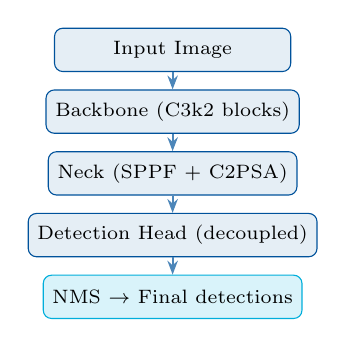
\begin{tikzpicture}[
          box/.style={draw=utecblue, fill=utecblue!10, rounded corners=3pt,
              minimum width=3.0cm, minimum height=0.55cm,
              font=\scriptsize, align=center},
          arr/.style={-{Stealth[length=5pt]}, utecblue!70, thick}
        ]
        \node[box] (img)  {Input Image};
        \node[box, below=0.22cm of img]  (bb)   {Backbone (C3k2 blocks)};
        \node[box, below=0.22cm of bb]   (neck) {Neck (SPPF + C2PSA)};
        \node[box, below=0.22cm of neck] (head) {Detection Head (decoupled)};
        \node[box, below=0.22cm of head, fill=uteccyan!15, draw=uteccyan]
        (nms)  {NMS $\to$ Final detections};
        \draw[arr] (img)  -- (bb);
        \draw[arr] (bb)   -- (neck);
        \draw[arr] (neck) -- (head);
        \draw[arr] (head) -- (nms);
      \end{tikzpicture}
    \end{column}
  \end{columns}
\end{frame}

% ── SLIDE 5: YOLO BACKBONE Y NECK ────────────────────────────────────────────
\begin{frame}{YOLOv11: Backbone and Neck}
  \begin{columns}[T]
    \begin{column}{0.48\textwidth}
      \textbf{Backbone --- C3k2 blocks:}
      \begin{itemize}
        \item Cross Stage Partial (CSP) with kernel size 2
        \item Splits feature maps into two branches:\\
              one processed, one bypassed $\to$ \textbf{fewer parameters}
        \item Progressive downsampling: $\frac{1}{8}$, $\frac{1}{16}$, $\frac{1}{32}$ of input
        \item Multi-scale feature extraction
      \end{itemize}
      \vspace{0.3em}
      \begin{block}{SPPF (Spatial Pyramid Pooling Fast)}
        \small Sequential $k\!\times\!k$ max-poolings concatenated,
        approximating multi-scale pooling at a single resolution
      \end{block}
    \end{column}
    \begin{column}{0.48\textwidth}
      \textbf{Neck --- C2PSA (key novelty of v11):}
      \begin{itemize}
        \item CSP block with \textbf{Positional Self-Attention}
        \item Attention weight for each position $(i,j)$:
      \end{itemize}
      \vspace{-0.2em}
      \[
        \mathrm{Attn}(Q,K,V)=
        \mathrm{softmax}\!\left(\frac{QK^\top}{\sqrt{d_k}}\right)V
      \]
      \begin{itemize}
        \item FPN (top-down) + PAN (bottom-up) feature fusion
        \item Combines semantic richness with spatial precision
      \end{itemize}
      \begin{alertblock}{}
        \scriptsize C2PSA adds global context without significant
        computational overhead compared to YOLOv8's C2f
      \end{alertblock}
    \end{column}
  \end{columns}
\end{frame}

% ── SLIDE 6: YOLO HEAD Y NMS ──────────────────────────────────────────────────
\begin{frame}{YOLOv11: Detection Head and NMS}
  \begin{columns}[T]
    \begin{column}{0.52\textwidth}
      \textbf{Decoupled detection head:}
      \begin{itemize}
        \item Separate branches for \textbf{classification} and
              \textbf{bounding-box regression}
        \item Avoids task-interference present in coupled heads
      \end{itemize}
      \vspace{0.3em}
      \textbf{Distribution Focal Loss (DFL) regression:}
      \begin{itemize}
        \item Predicts a \textbf{probability distribution} over
              discrete offsets, not a single point:
      \end{itemize}
      \[
        \hat{b} = \sum_{i=0}^{n-1} i \cdot P(b=i),
        \quad P = \mathrm{softmax}(\mathbf{z})
      \]
      \begin{itemize}
        \item Captures ambiguity in object boundary localization
      \end{itemize}
    \end{column}
    \begin{column}{0.44\textwidth}
      \textbf{Non-Maximum Suppression (NMS):}
      \begin{itemize}
        \item Removes redundant overlapping detections
        \item Keep box $b_i$ if $\nexists\, b_j$ with
              $\mathrm{conf}(b_j)>\mathrm{conf}(b_i)$ and
              $\mathrm{IoU}(b_i,b_j)>\tau_\mathrm{nms}$
      \end{itemize}
      \vspace{0.3em}
      \begin{block}{Inference hyperparameters}
        \small
        \texttt{conf} $= 0.25$\quad (detection threshold)\\
        \texttt{iou\_nms} $= 0.45$\quad (NMS threshold)\\
        \texttt{imgsz} $= 1280$\quad (input resolution)\\
        \texttt{device} $= \mathrm{GPU}$\quad (NVIDIA T4)
      \end{block}
    \end{column}
  \end{columns}
\end{frame}

% ── SLIDE 7: SORT VISIÓN GENERAL ──────────────────────────────────────────────
\begin{frame}{SORT: Simple Online and Realtime Tracking}
  \begin{columns}[T]
    \begin{column}{0.52\textwidth}
      \textbf{Bewley et al., ICIP 2016 \cite{bewley2016sort}:}
      \begin{itemize}
        \item Tracking-by-detection paradigm: tracker receives
              bboxes from the detector, does not re-detect
        \item \textbf{No visual appearance features} --- purely geometric
        \item Two classical components:
              \begin{itemize}
                \item \textbf{Kalman Filter}: motion prediction
                \item \textbf{Hungarian Algorithm}: optimal assignment
              \end{itemize}
        \item Achieves $>\!260$ FPS on tracking alone
      \end{itemize}
      \vspace{0.3em}
      \begin{alertblock}{Why SORT as baseline?}
        \small Its limitations (long occlusion, appearance ambiguity,
        tiny objects) directly motivate Methods 2--4.
      \end{alertblock}
    \end{column}
    \begin{column}{0.44\textwidth}
      \vspace{0.2cm}
      \begin{tikzpicture}[
          box/.style={draw=utecblue, fill=utecblue!10, rounded corners=3pt,
              minimum width=3.0cm, minimum height=0.55cm,
              font=\scriptsize, align=center},
          arr/.style={-{Stealth[length=5pt]}, utecblue!70, thick}
        ]
        \node[box] (det)  {Detections $\{b_i^t\}$};
        \node[box, below=0.22cm of det]  (pred) {① Kalman Predict};
        \node[box, below=0.22cm of pred] (iou)  {② IoU Cost Matrix};
        \node[box, below=0.22cm of iou]  (hung) {③ Hungarian Assignment};
        \node[box, below=0.22cm of hung] (upd)  {④ Update / Create / Delete};
        \node[box, below=0.22cm of upd, fill=uteccyan!15, draw=uteccyan]
        (out)  {Tracks $\{\tau_k^t\}$};
        \draw[arr] (det)  -- (pred);
        \draw[arr] (pred) -- (iou);
        \draw[arr] (iou)  -- (hung);
        \draw[arr] (hung) -- (upd);
        \draw[arr] (upd)  -- (out);
      \end{tikzpicture}
    \end{column}
  \end{columns}
\end{frame}

% ── SLIDE 8: SORT FILTRO DE KALMAN ────────────────────────────────────────────
\begin{frame}{SORT: Kalman Filter for Motion Prediction}
  \textbf{State vector} (7-dimensional, one Kalman filter per track):
  \[
    \mathbf{x} = \bigl[c_x,\; c_y,\; s,\; r,\; \dot{c}_x,\; \dot{c}_y,\; \dot{s}\bigr]^\top
  \]
  where $c_x, c_y$: bbox centre $\cdot$ $s = w \cdot h$: area $\cdot$
  $r = w/h$: aspect ratio (assumed constant) $\cdot$ $\dot{(\cdot)}$: velocity

  \begin{columns}[T]
    \begin{column}{0.48\textwidth}
      \textbf{Prediction step} (before observing detections):
      \[
        \mathbf{x}^-_t = F\,\mathbf{x}_{t-1}, \qquad
        P^-_t = F P_{t-1} F^\top + Q
      \]
      $F$: constant-velocity transition matrix \quad
      $P$: state covariance \quad $Q$: process noise
    \end{column}
    \begin{column}{0.48\textwidth}
      \textbf{Update step} (after associating a detection $\mathbf{z}=[c_x,c_y,s,r]^\top$):
      \[
        K = P^-_t H^\top\!\bigl(H P^-_t H^\top + R\bigr)^{-1}
      \]
      \[
        \mathbf{x}_t = \mathbf{x}^-_t + K\!\left(\mathbf{z} - H\mathbf{x}^-_t\right),
        \quad P_t = (I - KH)\,P^-_t
      \]
      $H$: observation matrix \quad $R$: measurement noise \quad
      $K$: Kalman gain (weights prediction vs.\ measurement)
    \end{column}
  \end{columns}
  \vspace{0.2em}
  \begin{block}{Intuition}
    \small If $K \to I$: trust the detection fully.
    If $K \to 0$: trust the prediction fully.
    $K$ is learned from the noise covariances $Q$ and $R$.
  \end{block}
\end{frame}

% ── SLIDE 9: SORT HÚNGARO Y GESTIÓN ───────────────────────────────────────────
\begin{frame}{SORT: Hungarian Assignment and Track Lifecycle}
  \begin{columns}[T]
    \begin{column}{0.50\textwidth}
      \textbf{IoU-based cost matrix:}
      \[
        C_{ij} = 1 - \mathrm{IoU}(\hat{\tau}_i,\, b_j^t)
      \]
      where $\hat{\tau}_i$: Kalman-predicted bbox of track $i$,\;
      $b_j^t$: detection $j$ at time $t$

      \textbf{Hungarian algorithm} minimises total cost:
      \[
        \sigma^* = \arg\min_{\sigma} \sum_i C_{i,\sigma(i)}
      \]
      Match rejected if $\mathrm{IoU} < \tau_\mathrm{IoU} = 0.3$
      \vspace{0.3em}
      \begin{alertblock}{Separate trackers per class}
        \small Independent SORT instances for pedestrians and cars
        prevent cross-class identity confusion.
      \end{alertblock}
    \end{column}
    \begin{column}{0.46\textwidth}
      \textbf{Track lifecycle:}
      \vspace{0.2em}

      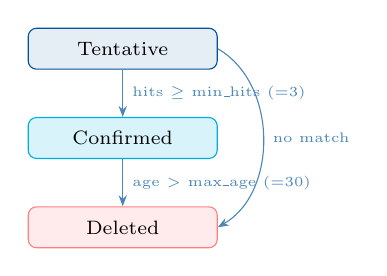
\begin{tikzpicture}[
          st/.style={draw=utecblue, rounded corners=3pt, fill=utecblue!10,
              minimum width=2.4cm, minimum height=0.52cm,
              font=\scriptsize, align=center},
          arr/.style={-{Stealth[length=4pt]}, utecblue!70}
        ]
        \node[st] (tent) {Tentative};
        \node[st, below=0.6cm of tent, fill=uteccyan!15, draw=uteccyan]
        (conf) {Confirmed};
        \node[st, below=0.6cm of conf, fill=red!8, draw=red!50]
        (dead) {Deleted};
        \draw[arr] (tent) -- node[right,font=\tiny]{hits $\geq$ min\_hits (=3)} (conf);
        \draw[arr] (conf) -- node[right,font=\tiny]{age $>$ max\_age (=30)} (dead);
        \draw[arr] (tent.east) to[bend left=60]
        node[right,font=\tiny]{no match} (dead.east);
      \end{tikzpicture}
      \vspace{0.2em}
      \begin{block}{}
        \scriptsize \texttt{min\_hits=3}: avoids spurious tracks from
        detector FPs.\quad
        \texttt{max\_age=30}: tolerates ${\sim}1$ s occlusions at 30 fps.
      \end{block}
    \end{column}
  \end{columns}
\end{frame}

% ── SLIDE 10: PIPELINE COMPLETO ───────────────────────────────────────────────
\begin{frame}{Full Pipeline: YOLOv11 + SORT}
  \centering
  \vspace{-0.2cm}
  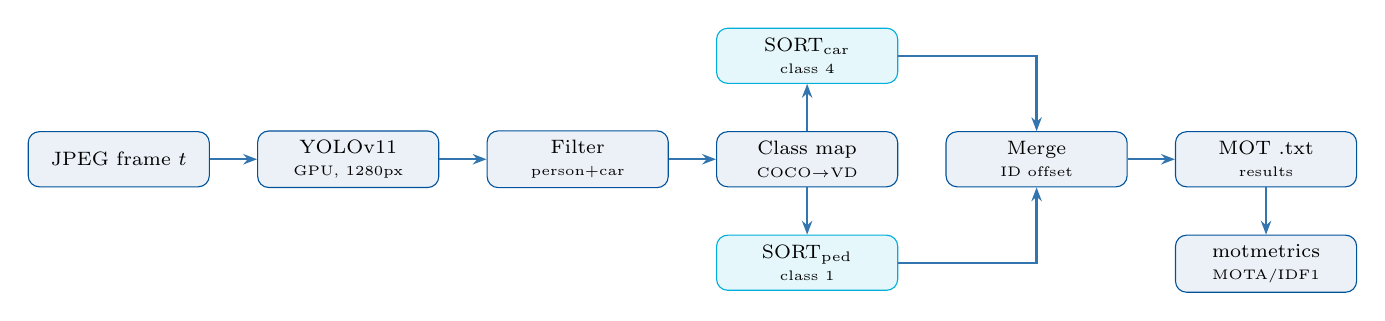
\begin{tikzpicture}[
      box/.style={draw=utecblue, fill=utecblue!8, rounded corners=4pt,
          minimum width=2.3cm, minimum height=0.7cm,
          font=\scriptsize, align=center},
      dbox/.style={draw=uteccyan, fill=uteccyan!10, rounded corners=4pt,
          minimum width=2.3cm, minimum height=0.7cm,
          font=\scriptsize, align=center},
      arr/.style={-{Stealth[length=5pt]}, utecblue!80, thick},
      note/.style={font=\tiny, text=utecblue!70, align=center}
    ]
    \node[box]  (fr)   {JPEG frame $t$};
    \node[box,  right=0.6cm of fr]  (yolo) {YOLOv11\\{\tiny GPU, 1280px}};
    \node[box,  right=0.6cm of yolo](filt) {Filter\\{\tiny person+car}};
    \node[box,  right=0.6cm of filt](map)  {Class map\\{\tiny COCO$\to$VD}};
    \node[dbox, below=0.6cm of map] (sp)   {SORT\textsubscript{ped}\\{\tiny class 1}};
    \node[dbox, above=0.6cm of map] (sc)   {SORT\textsubscript{car}\\{\tiny class 4}};
    \node[box,  right=0.6cm of map] (merge){Merge\\{\tiny ID offset}};
    \node[box,  right=0.6cm of merge](mot) {MOT .txt\\{\tiny results}};
    \node[box,  below=0.6cm of mot] (eval) {motmetrics\\{\tiny MOTA/IDF1}};

    \draw[arr] (fr)   -- (yolo);
    \draw[arr] (yolo) -- (filt);
    \draw[arr] (filt) -- (map);
    \draw[arr] (map.south) -- (sp.north);
    \draw[arr] (map.north) -- (sc.south);
    \draw[arr] (sp.east)   -| (merge.south);
    \draw[arr] (sc.east)   -| (merge.north);
    \draw[arr] (merge) -- (mot);
    \draw[arr] (mot.south) -- (eval.north);
  \end{tikzpicture}

  \vspace{0.4em}
  \begin{columns}[T]
    \begin{column}{0.48\textwidth}
      \begin{block}{Key design choice}
        \small Separate SORT trackers per class.
        Car IDs offset by $+100\,000$ to prevent
        ID collision across classes in the output file.
      \end{block}
    \end{column}
    \begin{column}{0.48\textwidth}
      \begin{block}{Output format (MOT standard)}
        \scriptsize
        \texttt{frame, id, x, y, w, h, conf, class, vis}\\
        One line per detection per frame.
        Sorted by \texttt{(frame, id)}.
      \end{block}
    \end{column}
  \end{columns}
\end{frame}

% ── SLIDE 11: MÉTRICAS ────────────────────────────────────────────────────────
\begin{frame}{Evaluation Protocol: MOT Metrics}
  \begin{columns}[T]
    \begin{column}{0.54\textwidth}
      \renewcommand{\arraystretch}{1.4}
      \small
      \begin{tabular}{p{1.0cm}p{5.3cm}}
        \toprule
        \textbf{Metric} & \textbf{Definition}                                       \\
        \midrule
        \textbf{MOTA}   &
        $1 - \dfrac{\mathrm{FP}+\mathrm{FN}+\mathrm{IDS}}{\sum_t |\mathcal{GT}_t|}$ \\[6pt]
        \textbf{MOTP}   &
        $\dfrac{\sum_{t,i} d_{t,i}}{\sum_t |\mathcal{M}_t|}$
        \;(avg.\ IoU of matched pairs)                                              \\[6pt]
        \textbf{IDF1}   &
        $\dfrac{2\,\mathrm{IDTP}}{2\,\mathrm{IDTP}+\mathrm{IDFP}+\mathrm{IDFN}}$    \\[6pt]
        \textbf{IDS}    & Total identity switches                                   \\
        \textbf{FPS}    & Frames per second (inference + assoc.)                    \\
        \bottomrule
      \end{tabular}
    \end{column}
    \begin{column}{0.42\textwidth}
      \textbf{Protocol settings:}
      \begin{itemize}
        \item Min.\ IoU for a TP match: $\tau=0.5$
        \item Classes: pedestrian (1) and car (4)
        \item GT annotations with \texttt{score=0} excluded
        \item Library: \texttt{motmetrics} (Python)
        \item NumPy 2.0 compatibility patch applied:\\
              {\scriptsize\texttt{np.asfarray} removed in NumPy 2.0}
      \end{itemize}
      \begin{alertblock}{Interpretation}
        \small MOTA $<0$ is possible when FP+FN+IDS exceeds
        the total number of GT objects.
      \end{alertblock}
    \end{column}
  \end{columns}
\end{frame}

% ── SLIDE 12: RESULTADOS POR SECUENCIA ────────────────────────────────────────
\begin{frame}{Quantitative Results by Sequence}
  \renewcommand{\arraystretch}{1.25}
  \small
  \begin{tabular}{lrrrrrr}
    \toprule
    \textbf{Sequence} & \textbf{MOTA}    & \textbf{IDF1}
                      & \textbf{IDS}     & \textbf{FP}      & \textbf{FN}      & \textbf{FPS}                  \\
    \midrule
    uav0000086        & 30.77\%          & 55.50\%          & 22               & 3\,432        & 6\,860 & 17.5 \\
    uav0000117        & 3.12\%           & 34.48\%          & 233              & 5\,107        & 6\,567 & 14.3 \\
    uav0000137        & 14.83\%          & 53.64\%          & 96               & 5\,788        & 2\,945 & 13.3 \\
    \rowcolor{red!10}
    uav0000182        & $-$26.25\%       & 42.20\%          & 47               & 5\,552        & 2\,851 & 15.6 \\
    uav0000268        & 8.40\%           & 24.91\%          & 12               & 1\,068        & 7\,694 & 18.0 \\
    \rowcolor{red!10}
    uav0000305        & 2.62\%           & 5.37\%           & 6                & 22            & 4\,021 & 17.9 \\
    uav0000339        & 18.14\%          & 41.37\%          & 79               & 2\,850        & 2\,179 & 15.5 \\
    \midrule
    \textbf{OVERALL}  & \textbf{10.58\%} & \textbf{42.66\%}
                      & \textbf{495}     & \textbf{23\,819} & \textbf{33\,117} & \textbf{16.0}                 \\
    \bottomrule
  \end{tabular}
  \vspace{0.4em}
  \begin{columns}[T]
    \begin{column}{0.48\textwidth}
      \begin{block}{Best sequence: uav0000086}
        \small Low resolution ($1344\!\times\!756$), relatively larger objects
        $\Rightarrow$ detector and IoU-matching work well
      \end{block}
    \end{column}
    \begin{column}{0.48\textwidth}
      \begin{alertblock}{Highlighted issues (red rows)}
        \small uav0000182: MOTA $<0$, excessive FP\\
        uav0000305: IDF1 $=5.37\%$, almost no tracked identity
      \end{alertblock}
    \end{column}
  \end{columns}
\end{frame}

% ── SLIDE 13: ANÁLISIS ────────────────────────────────────────────────────────
\begin{frame}{Results Analysis}
  \begin{columns}[T]
    \begin{column}{0.48\textwidth}
      \textbf{What worked}
      \begin{itemize}
        \item \textbf{uav0000086}: stable tracks, IDF1 $=55\%$,
              low IDS (22) — objects large enough for IoU matching
        \item \textbf{uav0000268}: fewest IDS (12) despite 4K resolution
              — sparse scene, less ambiguity
        \item SORT runs at $\sim$16 FPS end-to-end including YOLOv11
              inference at 1280 px on T4 GPU
      \end{itemize}
    \end{column}
    \begin{column}{0.48\textwidth}
      \textbf{What failed and why}
      \begin{itemize}
        \item \textbf{uav0000182}: MOTA $=-26\%$
              $\Rightarrow$ FP+FN+IDS $>$ GT count;
              dense scene, many background false positives
        \item \textbf{uav0000305}: IDF1 $=5.4\%$
              $\Rightarrow$ 41 of 41 GT trajectories \textbf{mostly lost};
              objects barely visible at native resolution
        \item \textbf{uav0000268} (4K, 978 frames):
              objects $<10$ px $\Rightarrow$ IoU $\approx 0$,
              SORT cannot associate detections
        \item 33\,117 FN total: detector misses most tiny objects
      \end{itemize}
    \end{column}
  \end{columns}
  \vspace{0.3em}
  \begin{block}{Root cause}
    \small YOLOv11 (COCO pre-trained) was not designed for sub-20 px aerial objects.
    IoU-only association breaks when bboxes are too small.
    Both problems are addressed by Methods 3 and 4.
  \end{block}
\end{frame}

% ── SLIDE 14: DEMO ÉXITO ──────────────────────────────────────────────────────
\begin{frame}{Qualitative Demo --- Success Case}
  \begin{columns}[T]
    \begin{column}{0.55\textwidth}
      \textbf{Sequence: uav0000086\_00000\_v}\\[4pt]
      {\small MOTA $=30.8\%$ \quad IDF1 $=55.5\%$ \quad IDS $=22$}
      \vspace{0.5em}
      \begin{itemize}
        \item Persistent track IDs across multiple frames
        \item Bounding boxes tightly fit pedestrians and cars
        \item Short occlusions recovered by Kalman prediction
        \item Low camera motion $\Rightarrow$ IoU matching effective
      \end{itemize}
      \vspace{0.4em}
      \begin{block}{Observation}
        \small When objects are $>\!40$ px, SORT's IoU-based
        association is sufficient for stable tracking.
      \end{block}
    \end{column}
    \begin{column}{0.42\textwidth}
      \centering
      %% ── PLACEHOLDER: replace with screenshot or frame crop ──────
      %% \includegraphics[width=\linewidth]{img/success_uav0000086.png}
      \imgplaceholder[5.5cm]{%
        \textbf{[IMAGE PLACEHOLDER]}\\[4pt]
        uav0000086\_00000\_v\\
        Frame with stable tracks\\
        Green = Car \quad Purple = Pedestrian\\[4pt]
        \footnotesize Insert frame screenshot\\
        or video still here
      }
    \end{column}
  \end{columns}
\end{frame}

% ── SLIDE 15: DEMO ÉXITO FRAMES ───────────────────────────────────────────────
\begin{frame}{Qualitative Demo --- Success Case (Track Continuity)}
  \begin{columns}[T]
    \begin{column}{0.32\textwidth}
      \centering
      {\small\textbf{Frame $t$}}\\[3pt]
      %% \includegraphics[width=\linewidth]{img/uav0086_t1.png}
      \imgplaceholder[3.5cm]{Frame $t$\\uav0000086}
    \end{column}
    \begin{column}{0.32\textwidth}
      \centering
      {\small\textbf{Frame $t+15$}}\\[3pt]
      %% \includegraphics[width=\linewidth]{img/uav0086_t2.png}
      \imgplaceholder[3.5cm]{Frame $t+15$\\same IDs}
    \end{column}
    \begin{column}{0.32\textwidth}
      \centering
      {\small\textbf{Frame $t+30$}}\\[3pt]
      %% \includegraphics[width=\linewidth]{img/uav0086_t3.png}
      \imgplaceholder[3.5cm]{Frame $t+30$\\IDs maintained}
    \end{column}
  \end{columns}
  \vspace{0.4em}
  \begin{block}{What to show}
    \small Same coloured bounding boxes and numeric IDs across the three
    frames, demonstrating that SORT maintains identity through motion.
  \end{block}
\end{frame}

% ── SLIDE 16: DEMO FALLO ──────────────────────────────────────────────────────
\begin{frame}{Qualitative Demo --- Failure Case}
  \begin{columns}[T]
    \begin{column}{0.55\textwidth}
      \textbf{Sequence: uav0000268\_05773\_v}\\[4pt]
      {\small MOTA $=8.4\%$ \quad IDF1 $=24.9\%$ \quad IDS $=12$\\
        Resolution: $3840\!\times\!2160$ (4K) \quad 978 frames}
      \vspace{0.4em}
      \begin{itemize}
        \item Objects appear as $5$--$10$ px blobs
        \item YOLOv11 (COCO) misses most of them $\Rightarrow$ 7\,694 FN
        \item $\mathrm{IoU}\!\approx\!0$ between tiny bboxes $\Rightarrow$
              SORT cannot associate detections
        \item Many spurious tracks from background noise
      \end{itemize}
      \vspace{0.3em}
      \begin{alertblock}{Motivation for Method 4 (SAHI)}
        \small Slicing Aided Hyper Inference tiles the image into
        overlapping crops, effectively upscaling tiny objects
        to a detectable size.
      \end{alertblock}
    \end{column}
    \begin{column}{0.42\textwidth}
      \centering
      %% ── PLACEHOLDER: replace with screenshot or frame crop ──────
      %% \includegraphics[width=\linewidth]{img/failure_uav0000268.png}
      \imgplaceholder[5.5cm]{%
        \textbf{[IMAGE PLACEHOLDER]}\\[4pt]
        uav0000268\_05773\_v\\
        4K frame --- tiny objects\\
        Missing detections / fragmented tracks\\[4pt]
        \footnotesize Insert frame screenshot\\
        or video still here
      }
    \end{column}
  \end{columns}
\end{frame}

% ── SLIDE 17: DEMO FALLO FRAMES ───────────────────────────────────────────────
\begin{frame}{Qualitative Demo --- Failure Case (ID Switch)}
  \begin{columns}[T]
    \begin{column}{0.32\textwidth}
      \centering
      {\small\textbf{Before occlusion}}\\[3pt]
      \imgplaceholder[3.5cm]{Track ID \#42\\clearly visible}
    \end{column}
    \begin{column}{0.32\textwidth}
      \centering
      {\small\textbf{During occlusion}}\\[3pt]
      \imgplaceholder[3.5cm]{Track lost\\(age $>$ max\_age)}
    \end{column}
    \begin{column}{0.32\textwidth}
      \centering
      {\small\textbf{After occlusion}}\\[3pt]
      \imgplaceholder[3.5cm]{New ID \#87\\assigned (IDS +1)}
    \end{column}
  \end{columns}
  \vspace{0.4em}
  \begin{alertblock}{Root cause of ID switch}
    \small When an object is occluded for $>\!$ \texttt{max\_age} frames,
    SORT deletes the track. On reappearance, no Kalman prediction
    is available $\Rightarrow$ a new ID is assigned.
    DeepSORT / BoT-SORT solve this with \textbf{appearance embeddings}.
  \end{alertblock}
\end{frame}

% ── SLIDE 18: LIMITACIONES Y MÉTODOS 2-4 ─────────────────────────────────────
\begin{frame}{Baseline Limitations and Motivation for Methods 2--4}
  \renewcommand{\arraystretch}{1.3}
  \small
  \begin{tabular}{p{3.0cm}p{4.0cm}p{4.5cm}}
    \toprule
    \textbf{Problem} & \textbf{Root cause}                           & \textbf{Solution} \\
    \midrule
    Tiny objects undetected
                     & COCO training; objects $<$20 px
                     & \textbf{Method 4}: SAHI tiling                                    \\
    ID switches at crossings
                     & IoU-only; no appearance model
                     & \textbf{Method 3}: BoT-SORT (ReID + GMC)                          \\
    Dense-scene FP
                     & NMS removes clustered detections
                     & \textbf{Method 2}: YOLO26 (NMS-free)                              \\
    FPS limited ($\sim$16)
                     & YOLOv11 at 1280 px dominates
                     & \textbf{Method 2}: YOLO26 (more efficient)                        \\
    Long-occlusion IDS (495 total)
                     & No visual re-ID; fixed max\_age
                     & \textbf{Method 3}: Global Motion Compensation                     \\
    \bottomrule
  \end{tabular}
  \vspace{0.4em}
  \begin{columns}[T]
    \begin{column}{0.48\textwidth}
      \begin{block}{Overall MOTA: 10.58\%}
        \small Acceptable for a geometry-only baseline on aerial data.
        IDF1 $=42.7\%$ shows partial identity retention.
      \end{block}
    \end{column}
    \begin{column}{0.48\textwidth}
      \begin{alertblock}{Expected improvement direction}
        \small Methods 2--4 address orthogonal failure modes;
        combined they should substantially raise MOTA and IDF1.
      \end{alertblock}
    \end{column}
  \end{columns}
\end{frame}

% ── SLIDE 19: REFERENCIAS ─────────────────────────────────────────────────────
\begin{frame}[allowframebreaks]{References}
  \footnotesize
  \begin{thebibliography}{9}

    \bibitem{zhu2022visdrone}
    P.~Zhu, L.~Wen, D.~Du, X.~Bian, H.~Fan, Q.~Hu, and H.~Ling,
    ``Detection and Tracking Meet Drones Challenge,''
    \textit{IEEE Transactions on Pattern Analysis and Machine Intelligence},
    vol.~44, no.~11, pp.~7380--7399, Nov.~2022.
    DOI: 10.1109/TPAMI.2021.3119563.

    \bibitem{bewley2016sort}
    A.~Bewley, Z.~Ge, L.~Ott, F.~Ramos, and B.~Upcroft,
    ``Simple Online and Realtime Tracking,''
    in \textit{Proc. IEEE Int. Conf. Image Processing (ICIP)},
    Phoenix, AZ, Sep.~2016, pp.~3464--3468.
    DOI: 10.1109/ICIP.2016.7533003.

    \bibitem{lin2014coco}
    T.-Y.~Lin, M.~Maire, S.~Belongie, J.~Hays, P.~Perona, D.~Ramanan,
    P.~Dollár, and C.~L.~Zitnick,
    ``Microsoft COCO: Common Objects in Context,''
    in \textit{Proc. European Conf. Computer Vision (ECCV)},
    Zurich, Switzerland, Sep.~2014, pp.~740--755.
    DOI: 10.1007/978-3-319-10602-1\_48.

    \bibitem{ultralytics2024yolo11}
    Ultralytics,
    ``YOLOv11: A Leap Forward in Real-Time Object Detection,''
    \textit{Ultralytics Documentation}, 2024.
      [Online]. Available: \url{https://docs.ultralytics.com/models/yolo11/}

    \bibitem{kalman1960}
    R.~E.~Kalman,
    ``A New Approach to Linear Filtering and Prediction Problems,''
    \textit{Journal of Basic Engineering},
    vol.~82, no.~1, pp.~35--45, Mar.~1960.
    DOI: 10.1115/1.3662552.

    \bibitem{kuhn1955hungarian}
    H.~W.~Kuhn,
    ``The Hungarian Method for the Assignment Problem,''
    \textit{Naval Research Logistics Quarterly},
    vol.~2, no.~1--2, pp.~83--97, 1955.
    DOI: 10.1002/nav.3800020109.

    \bibitem{wojke2017deepsort}
    N.~Wojke, A.~Bewley, and D.~Paulus,
    ``Simple Online and Realtime Tracking with a Deep Association Metric,''
    in \textit{Proc. IEEE Int. Conf. Image Processing (ICIP)},
    Beijing, China, Sep.~2017, pp.~3645--3649.
    DOI: 10.1109/ICIP.2017.8296962.

    \bibitem{aharon2022botsort}
    N.~Aharon, R.~Orfaig, and B.-Z.~Bobrovsky,
    ``BoT-SORT: Robust Associations Multi-Pedestrian Tracking,''
    \textit{arXiv preprint arXiv:2206.14651}, Jun.~2022.
      [Online]. Available: \url{https://arxiv.org/abs/2206.14651}

    \bibitem{akbari2022sahi}
    O.~F.~Cengiz, F.~Akyon, E.~Altinuc, and A.~Tekin,
    ``Slicing Aided Hyper Inference and Fine-tuning for
    Small Object Detection,''
    in \textit{Proc. IEEE Int. Conf. Image Processing (ICIP)},
    Bordeaux, France, Oct.~2022, pp.~966--970.
    DOI: 10.1109/ICIP46576.2022.9897990.

  \end{thebibliography}
\end{frame}

% ── SLIDE 20: CIERRE ──────────────────────────────────────────────────────────
{
  \setbeamercolor{background canvas}{bg=utecblue}
  \begin{frame}[plain]
    \centering
    \vspace{2cm}
    {\color{white}\Huge\bfseries Thank you\par}
    \vspace{0.8em}
    {\color{uteccyan}\large Questions?\par}
    \vspace{1.5em}
    {\color{white!70}Computer Vision --- UTEC, 2026-I\par}
    \vspace{0.3em}
    {\color{white!50}\small Assignment IV: Detection and Tracking --- Method 1 Baseline\par}
  \end{frame}
}

\end{document}